%%%%%%%%%%%%%%%%%%%%%%%%%%%%%%%%%%%%%%%%%
% baposter Portrait Poster
% LaTeX Template
% Version 1.0 (15/5/13)
%
% Created by:
% Brian Amberg (baposter@brian-amberg.de)
%
% This template has been downloaded from:
% http://www.LaTeXTemplates.com
%
% License:
% CC BY-NC-SA 3.0 (http://creativecommons.org/licenses/by-nc-sa/3.0/)
%
%%%%%%%%%%%%%%%%%%%%%%%%%%%%%%%%%%%%%%%%%

%----------------------------------------------------------------------------------------
%	PACKAGES AND OTHER DOCUMENT CONFIGURATIONS
%----------------------------------------------------------------------------------------

\documentclass[b0paper,portrait]{baposter}
\usepackage{comment}
\usepackage{tikz}
\usepackage[font=small,labelfont=bf]{caption} % Required for specifying captions to tables and figures
\usepackage{booktabs} % Horizontal rules in tables
\usepackage{relsize} % Used for making text smaller in some places
\usepackage{amsfonts}
\usepackage{amsmath, bm}
\usepackage{hyperref}
\usepackage{pgfplots}
\usepackage{graphicx}
%\usepackage{wrapfig}
\usepackage{multicol}
\usepackage{array}
\usepackage{subfig}
\usepackage{url}
\usepackage[export]{adjustbox}
\usetikzlibrary{positioning}
%\usepgfplotslibrary{patchplots}
%\pgfplotsset{compat=newest}

\graphicspath{{figures/}} % Directory in which figures are stored


\makeatletter
\protected\def\vvv#1{\leavevmode\bgroup\vbox\bgroup\xvvv#1\relax}

\def\xvvv{\afterassignment\xxvvv\let\tmp= }

\def\xxvvv{%
\ifx\tmp\@sptoken\egroup\ \vbox\bgroup\let\next\xvvv
\else\ifx\tmp\relax\egroup\egroup\let\next\relax
\else
%\hbox{\tmp}%original
\hbox to 1.1em{\hfill\tmp\hfill}% centred
\let\next\xvvv\fi\fi
\next}

\makeatother

\definecolor{bordercol}{RGB}{40,40,40} % Border color of content boxes
\definecolor{headercol1}{RGB}{171,205, 239}%{186,215,230} % Background color for the header in the content boxes (left side)
\definecolor{headercol2}{RGB}{192, 192, 192}%{80,80,80} % Background color for the header in the content boxes (right side)
\definecolor{headerfontcol}{RGB}{0,0,0} % Text color for the header text in the content boxes
\definecolor{boxcolor}{RGB}{186,215,230} % Background color for the content in the content boxe
%\definecolor{airforceblue}{rgb}{0.36, 0.54, 0.66}


\definecolor{bluemathlab}{HTML}{065895}
\definecolor{orangemathlab}{HTML}{F79A25}
\newcommand{\highlight}[1]{\textbf{\color{bluemathlab}#1}}
\newcommand{\highlightB}[1]{\textbf{\color{black!15!orangemathlab}#1}}
\newcommand{\rbnics}{\highlightB{\texttt{RB}}\highlight{\texttt{niCS}}}
\newcommand{\fenics}{\texttt{FEniCS}}
\newcommand{\ped}[1]{_{\mathrm{#1}}}
\newcommand{\up}[1]{^{\mathrm{#1}}}
\renewcommand{\r}{\mathbf{r}}
\renewcommand{\d}{\mathrm{d}}
\newcommand{\x}{\times}
\newcommand{\dund}[1]{\underline{\underline{#1}}}
\newcommand{\und}[1]{\underline{#1}}
\newcommand{\mmu}{\boldsymbol\mu}

\def\Put(#1,#2)#3{\leavevmode\makebox(0,0){\put(#1,#2){#3}}}
\usepackage[procnames]{listings}

\definecolor{keywords}{RGB}{255,0,90}
\definecolor{comments}{RGB}{0,0,113}
\definecolor{red}{RGB}{160,0,0}
\definecolor{green}{RGB}{0,150,0}
\definecolor{mygray}{rgb}{0.5,0.5,0.5}

\lstset{language=Python, 
        basicstyle=\ttfamily\small, 
        keywordstyle=\color{keywords},
        commentstyle=\color{comments},
        stringstyle=\color{red},
        showstringspaces=false,
        identifierstyle=\color{green},
        procnamekeys={def,class},
		breaklines=true,
%    	postbreak={\ensuremath{\color{red}\hookrightarrow}},
  numbers=left,                    % where to put the line-numbers; possible values are (none, left, right)
  numbersep=-5pt,                   % how far the line-numbers are from the code
  numberstyle=\tiny\color{mygray}, % the style that is used for the line-numbers
}

\begin{document}

\background{ % Set the background to an image (background.pdf)
\begin{tikzpicture}[remember picture,overlay]
\draw (current page.north west)+(-2em,2em) node[anchor=north west]
{
\includegraphics[height=1.1\textheight]{background.png}};
\end{tikzpicture}
}

\begin{poster}{
grid=false,
borderColor=bordercol, % Border color of content boxes
headerColorOne=headercol1, % Background color for the header in the content boxes (left side)
headerColorTwo=headercol2, % Background color for the header in the content boxes (right side)
headerFontColor=headerfontcol, % Text color for the header text in the content boxes
boxColorOne= white,%boxcolor, % Background color for the content in the content boxes
%headershape=rounded,%right, % Specify the rounded corner in the content box headers
headerfont=\Large\sf\bf, % Font modifiers for the text in the content box headers
textborder=rectangle,
background=user,
headerborder=closed, % Change to closed for a line under the content box headers
boxshade=plain,
columns=6,
headerheight=0.1\textheight
}
{%
%\hspace{.2cm}
}%{
\includegraphics[height=3.5em]{erc}\hspace{.2cm}\includegraphics[height=7.5em]{aroma-logo}}
%
%----------------------------------------------------------------------------------------
%	TITLE AND AUTHOR NAME
%----------------------------------------------------------------------------------------
%
{\\\vspace{0.25cm} {\huge\bf Machine Learning and Optimal Transport \\ \vspace{0.25cm} for shape parametrisation}} % Poster title
{\vspace{0.25cm} Guglielmo Padula, Francesco Romor, Giovanni Stabile, Nicola Demo, Gianluigi Rozza \\ % Author names
{\smaller \vspace{0.25cm} Mathematics Area, mathLab, SISSA, International School of Advanced Studies, Trieste, Italy}
} % Author email addresses
{
} % University/lab logo
\Put(70,2200){
\includegraphics[height=6em]{logo_sissa_cerchio.png}}
\Put(0,2200){
\includegraphics[height=6em]{logo-mathlab_no_borders}}
\Put(665,2200){
\includegraphics[height=6em]{logo_uni}}
\Put(735,2200){
\includegraphics[height=6em]{logo_dssc}}

%----------------------------------------------------------------------------------------

\headerbox{Introduction: 2 lines of research}{name=introduction,column=0,row=0,span=6}{
\hspace{.2cm}
\begin{minipage}{0.47\textwidth} First line consist in studying  \textbf{generative models} for shape optimization of complex geometries with a large number of parameters; the objective is to learn the shape of the geometry using a minor number of parameters, for example for modeling naval hulls, and creating new artificial geometries similar to real data, as creating new real geometries can be costly.
\end{minipage}
\hspace{.2cm}
\begin{minipage}{0.47\textwidth}
In the second line \textbf{semidiscrete optimal transport} is used to obtain an optimal transport map to find some intermediate geometries with some regularity constraints. An application is design optimization, in which the quantity of material for similar models must be the same. The extension of semidiscrete optimal transport to three meshes will also be discussed.
\end{minipage}
}


%----------------------------------------------------------------------------------------

%----------------------------------------------------------------------------------------

\begin{posterbox}[name=otm,below=introduction,span=6,column=0]{2
    - Optimal Transport }
%\vspace{-0.5cm}
\hspace{.2cm}
\begin{minipage}{0.48\textwidth}
Given $\Omega$ a Borel set and two measures $\mu$ and $\nu$ on $\Omega$ such that $\mu(\Omega)=\nu(\Omega)$, $c$ a convex function $T: \Omega \rightarrow \Omega$ such that $$\begin{cases} \nu(X)=\mu(T^{-1}(X)) \quad \text{for any Borel (i.e. measurable) subset $X$ of $\Omega$}\\  \int_{\Omega} c(x, T(x)) d \mu \quad \text { is minimal }\end{cases}$$\\ is called the \textbf{optimal transport} map from $\mu$ to $\nu$.
We are interested in $\mu$ continuos and $\nu$ discrete. It this case we talk of Semi Discrete Optimal Transport.\\
\\We can approximate the optimal transport map with the following algorithm:\\
$\null$\\
Data: Two tetrahedral meshes $M$ and $M^{\prime}$, and $k$ the desired number of vertices in the result\\
Result: A tetrahedral mesh $G$ with $k$ vertices and a pair of points $p_{i}^{0}$ and $p_{i}^{1}$ attached to each vertex. Transport is parameterized by time $t \in[0,1]$ with $p_{i}(t)=(1-t) p_{i}^{0}+t p_{i}^{1}$.\\
(1) Sample $M^{\prime}$ with a set $Y$ of $k$ points\\
(2) Compute the weight vector $W$ that realizes the optimal transport between $M$ and $Y$\\
(3) Construct $E=Del(Y)$ where $Del$ it the Delaunay Triangulation.\\
(4) For each $i \in[1 \ldots k],\left(p_{i}\right)^{0} \leftarrow \operatorname{centroid}\left(\operatorname{Pow}_{W}\left(y_{i}\right) \cap M\right) $ , $\quad\left(p_{i}\right)^{1} \leftarrow y_{i}$\\
G will be the mesh defined by the topology of $E$ with the pair of points $(p_{i})^{0}$,$(p_{i})^{1}$.
It can be proven that the linear map does not clash particles. This algorithm is implemented in the library \textbf{Geogram} created by Bruno Levy.\\
We modified the map to be  $$\phi_{MM^{\prime}} (t)= {Vol(M)}^{\frac{1}{3}}\frac{tM^{\prime}+(1-t)M}{Vol(tM^{\prime}+(1-t)M)^{\frac{1}{3}}}$$
in order to preserve volume in intermediate times.\\
\end{minipage}
\hspace{.2cm}
\begin{minipage}{0.46\textwidth}
Let $M$, $M^{\prime}$, $M^{\prime\prime}$ three meshes. Let us suppose we calculate the OTM from $M$ to $M^{\prime}$ and from $M^{\prime\prime}$ selecting  $M^{\prime}$ to be sampled in the same way in both transports, so the resulting mesh will be the same (because in the algorithm does not depend on the other).  
So with the same assumption as before we can define a new transport map $$\phi_{MM^{\prime}M^{(2)}}(t)=\begin{cases}
Vol(M^{\prime})^{\frac{1}{3}}\frac{2tM^{\prime}+(1-2t)M}{Vol(2tM^{\prime}+(1-2t)M)^{\frac{1}{3}}} & 0 \le t \le \frac{1}{2} \\
Vol(M^{\prime})^{\frac{1}{3}}\frac{(2t-1)M^{\prime\prime}+(2-2t)M^{\prime}}{Vol((2t-1)M^{\prime\prime}+(2-2t)M^{\prime})^{\frac{1}{3}}} & \frac{1}{2} \le t \le 1
\end{cases}$$
that goes from $M$ to $M^{\prime}$ and then from $M^{\prime}$ to $M^{\prime\prime}$.  \\
Here is showed an example of three mesh OTM of a Bulbous bow, the three meshes are images in odd position, while in even position we have the intermediate meshes:
\begin{center}
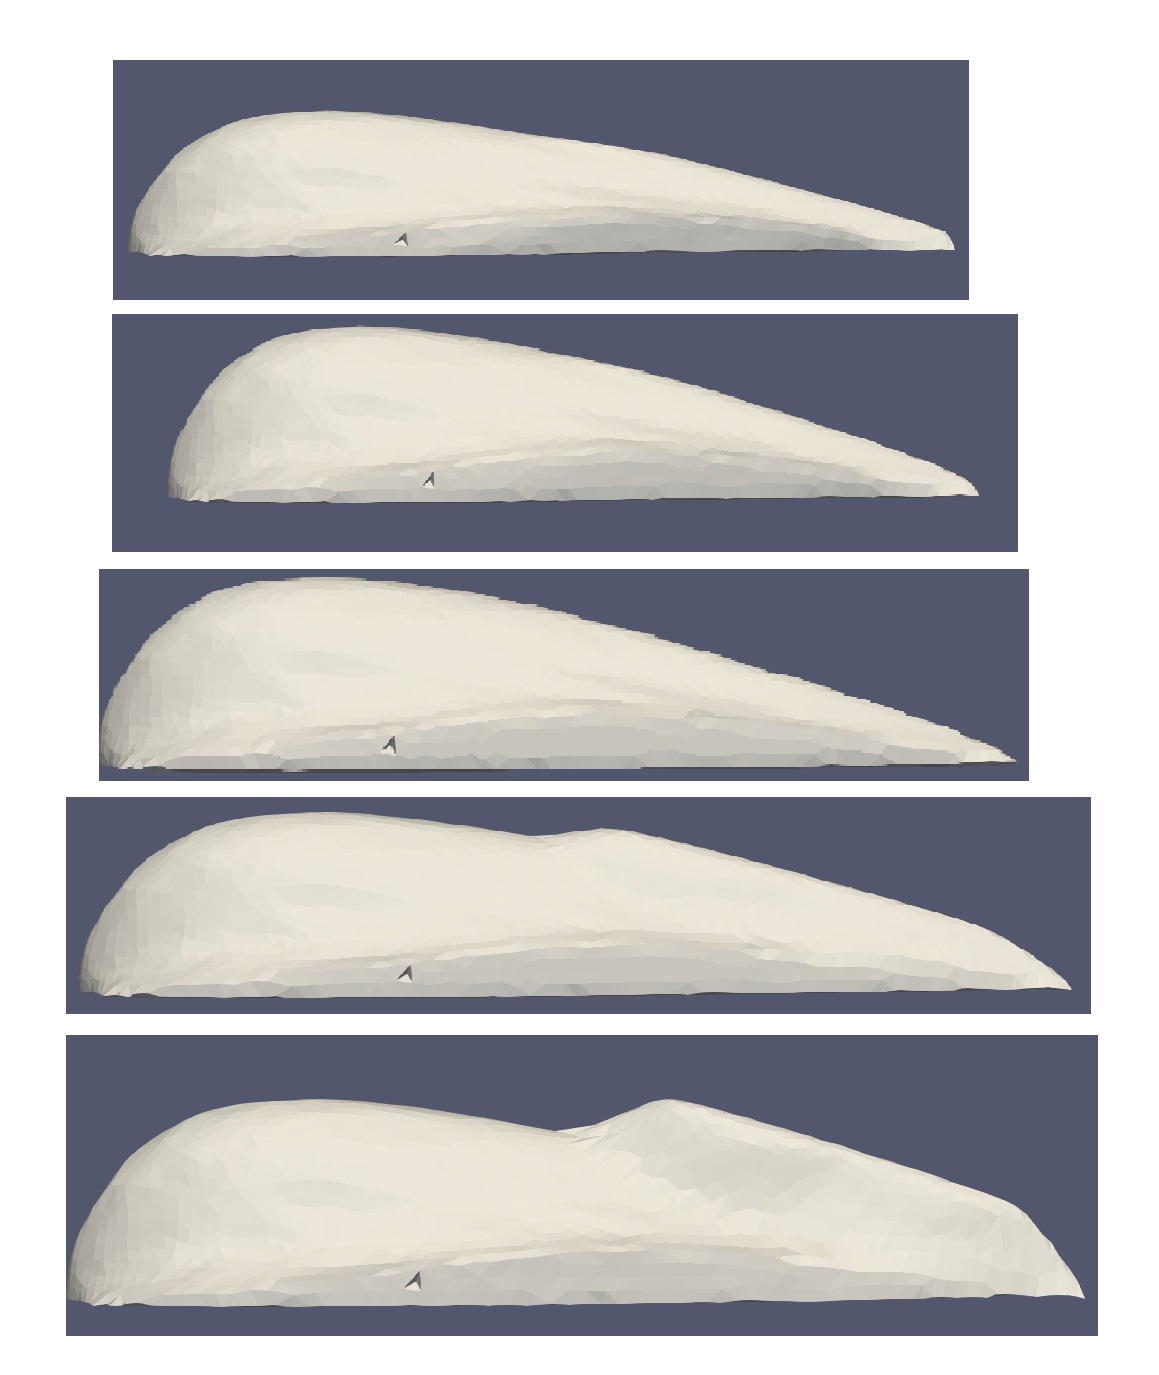
\includegraphics[scale=0.3]{otm2} 
\end{center}
\end{minipage}
\end{posterbox}

\begin{posterbox}[name=vae,below=otm,span=6,column=0]{4
    - Generative Models }
Two main model classes:
\begin{itemize}
\item Variational autoencoders: figure a) describes the training using a point cloud mesh of Bulbous bow, and figure b) shows sampling of a deformed Bulbous\\
a)\begin{tikzpicture}[thick,scale=0.7, every node/.style={scale=0.7},
squarednode/.style={rectangle, draw=blue!60, fill=red!5, very thick, minimum size=5mm},
]
\node[inner sep=0pt] (p11) {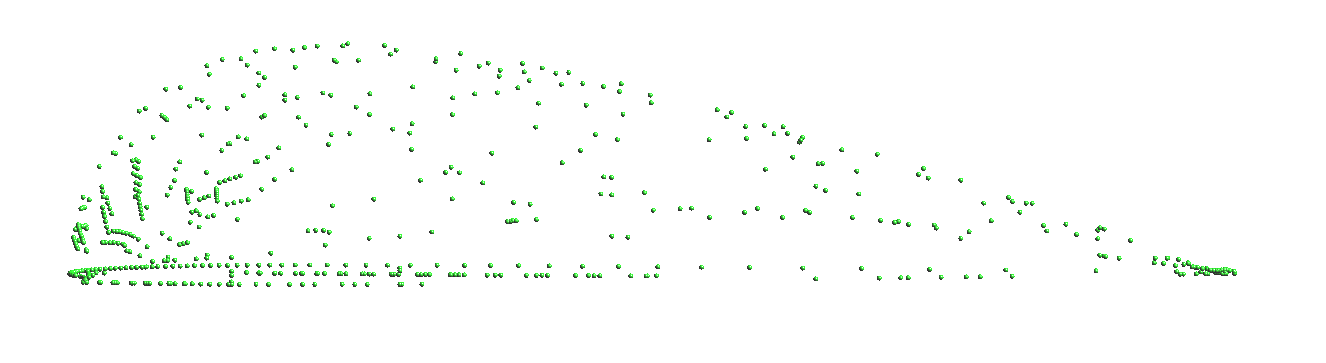
\includegraphics[scale=0.10]{p1}};
\node[squarednode]      (encoder)       [right=of p11]{\vvv{ENCODER}};
\node[inner sep=0pt] (normal)  [right=of encoder]{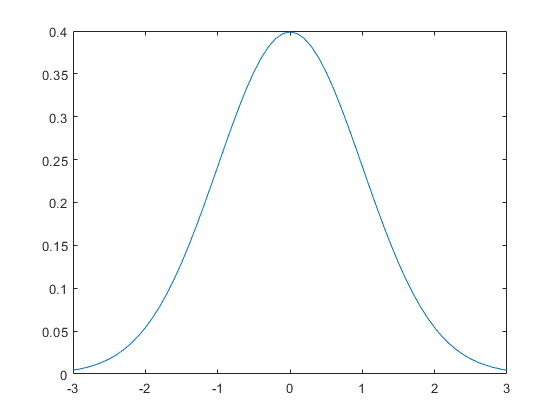
\includegraphics[scale=0.15]{normal}};
\node[squarednode]      (decoder)       [right=of normal]{\vvv{DECODER}};
\node[inner sep=0pt] (p21) [right=of decoder]{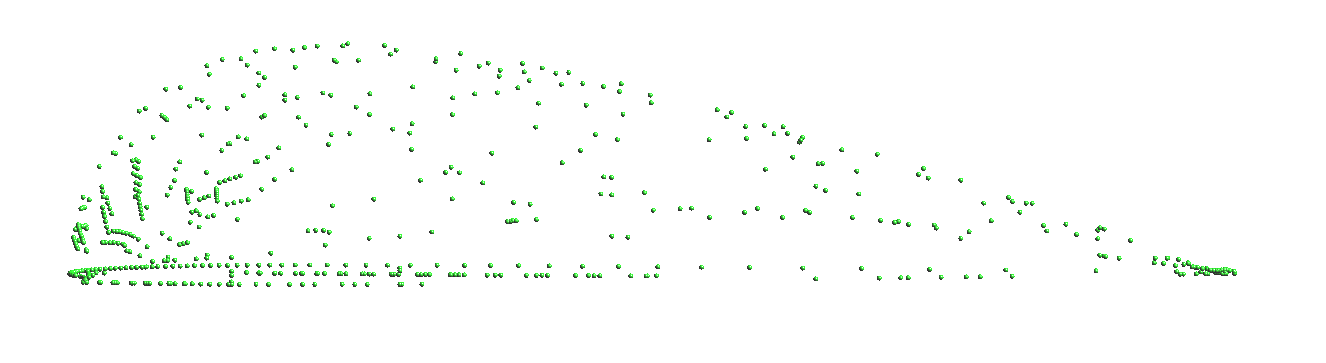
\includegraphics[scale=0.10]{p1}};

\draw[->] (p11.east) -- (encoder.west);
\draw[->] (encoder.east) -- (normal.west);
\draw[->] (normal.east) -- (decoder.west);
\draw[->] (decoder.east) -- (p21.west);
\end{tikzpicture}\qquad \qquad b) \begin{tikzpicture}[thick,scale=0.7, every node/.style={scale=0.7},
squarednode/.style={rectangle, draw=blue!60, fill=red!5, very thick, minimum size=5mm},
]
\node[inner sep=0pt] (normal)  {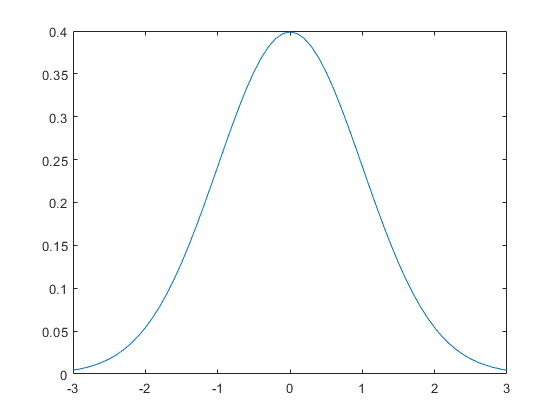
\includegraphics[scale=0.15]{normal}};
\node[squarednode]      (decoder)       [right=of normal]{\vvv{DECODER}};
\node[inner sep=0pt] (p21) [right=of decoder]{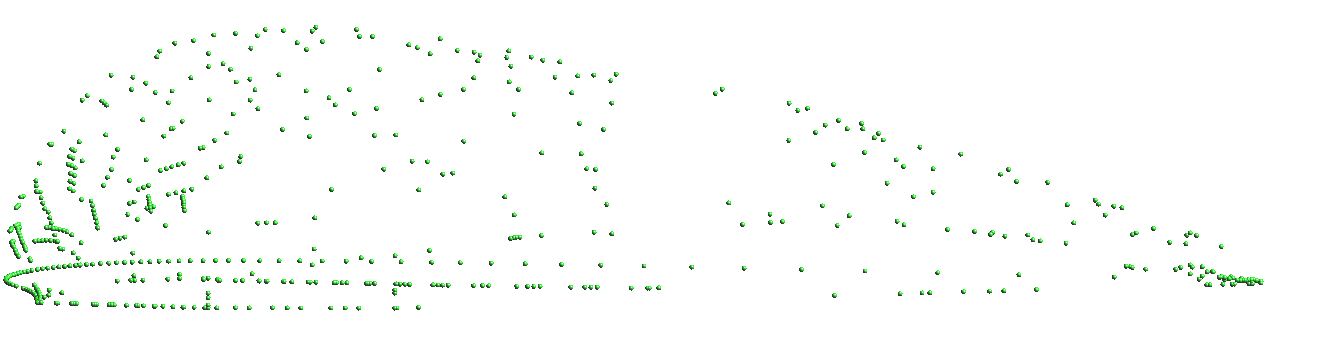
\includegraphics[scale=0.10]{p2}};

\draw[->] (normal.east) -- (decoder.west);
\draw[->] (decoder.east) -- (p21.west);
\end{tikzpicture}


\item Generative adversarial network:it is characterized by a generator that samples point cloud mesh of deformed Bulbous bow and by a discriminator that accepts real Bulbous (figure b)) and rejects deformed ones (figure a)).  \\
a)\begin{tikzpicture}[thick,scale=0.7, every node/.style={scale=0.7},
bluesquarednode/.style={rectangle, draw=blue!60, fill=red!5, very thick, minimum size=5mm},
redsquarednode/.style={rectangle, draw=red!60, fill=red!5, very thick, minimum size=5mm},]


\node[inner sep=0pt] (normal) {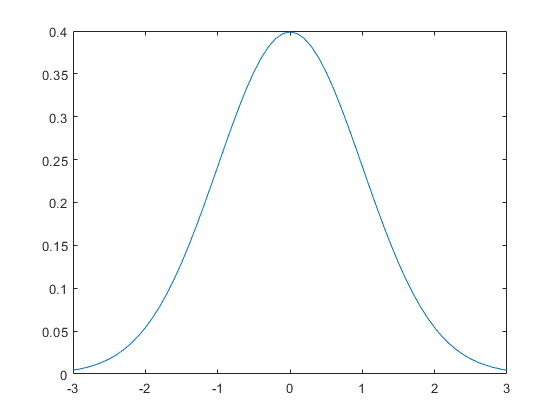
\includegraphics[scale=0.10]{normal}};
\node[bluesquarednode]      (generator)       [right=of normal]{\vvv{GENERATOR}};
\node[inner sep=0pt] (mesh)  [right=of generator]{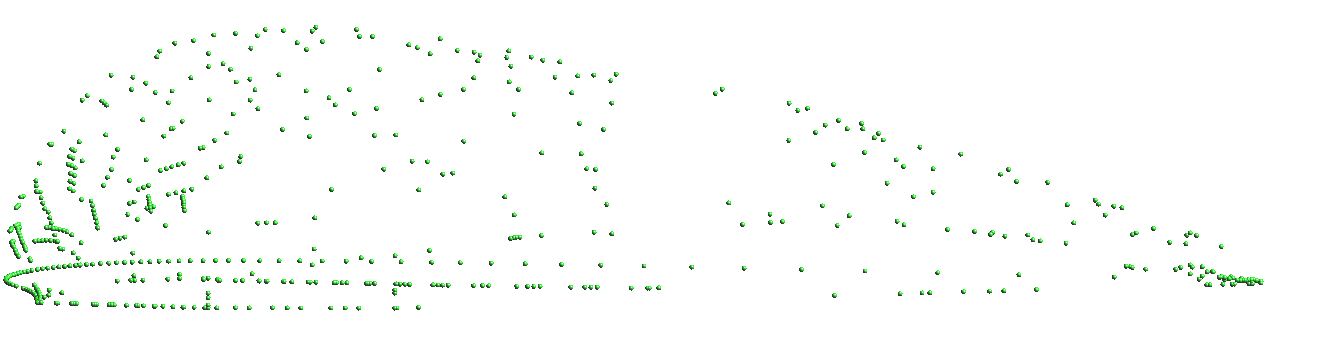
\includegraphics[scale=0.15]{p2}};
\node[bluesquarednode]      (discriminator)       [right=of mesh]{\vvv{DISCRIMINATOR}};
\node[redsquarednode]      (false)       [right=of discriminator]{FALSE};

\draw[->] (normal.east) -- (generator.west);
\draw[->] (generator.east) -- (mesh.west);
\draw[->] (mesh.east) -- (discriminator.west);
\draw[->] (discriminator.east) -- (false.west);
\end{tikzpicture}\qquad \qquad b)\begin{tikzpicture}[thick,scale=0.7, every node/.style={scale=0.7},
bluesquarednode/.style={rectangle, draw=blue!60, fill=red!5, very thick, minimum size=5mm},
greensquarednode/.style={rectangle, draw=green!60, fill=green!5, very thick, minimum size=5mm},]


\node[inner sep=0pt] (cad)  {
\includegraphics[scale=0.15]{cad}};
\node[inner sep=0pt] (mesh)  [right=of cad]{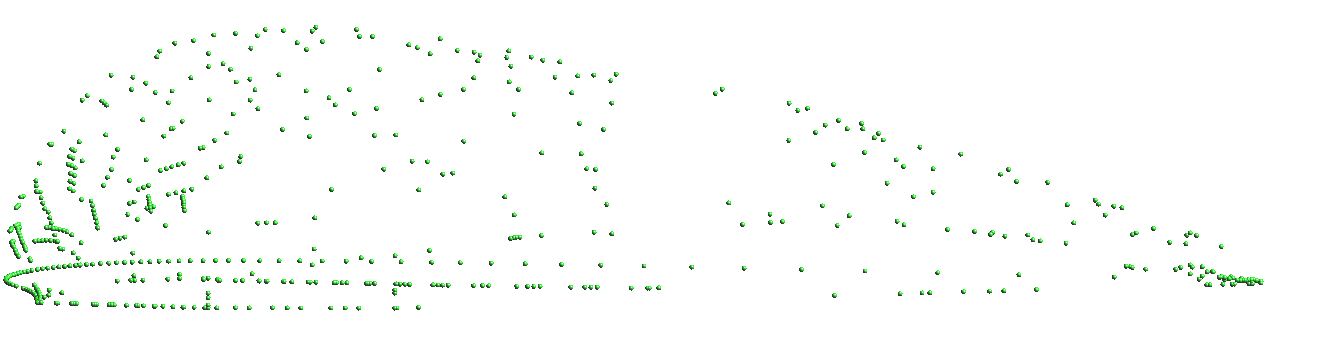
\includegraphics[scale=0.15]{p2}};
\node[bluesquarednode]      (discriminator)       [right=of mesh]{\vvv{DISCRIMINATOR}};
\node[greensquarednode]      (false)       [right=of discriminator]{TRUE};

\draw[->] (cad.east) -- (mesh.west);
\draw[->] (mesh.east) -- (discriminator.west);
\draw[->] (discriminator.east) -- (false.west);
\end{tikzpicture}


\end{itemize}
\end{posterbox}
\begin{posterbox}[name=results,below=vae,span=6,column=0]{5
    - Preliminary results and future work}
Summary of our results:
\begin{itemize}
\item We are able to do volume preserving continuos deformation between three bulbous bows meshes using semidiscrete optimal trasport. Our next step is to generalize it for more than three meshes, which is nontrivial (as $M$ and $M^{\prime}$ are nonsampled).
\item We are able to sample bulbous bows meshes using Variational Autoencoders. However, the space $Z$ is too much sparse, so we started studying Generative Adversarial Networks. 
\end{itemize}
\end{posterbox}
\begin{posterbox}[name=bibliography,below=results,span=6,column=0]{Bibliography and Software References}
\begin{itemize}
\item Geogram, \url{http://alice.loria.fr/software/geogram/doc/html/index.html}
\item A numerical algorithm for $L_{2}$ semi-discrete optimal transport in 3D, Bruno Levy, arXiv, 2014
\item Variational Autoencoders for Deforming 3D Mesh Models, Qingyang Tan, arXiv, 2018
\end{itemize}
\end{posterbox}

\end{poster}

\end{document}
